

\tikzset{every picture/.style={line width=0.75pt}} %set default line width to 0.75pt        

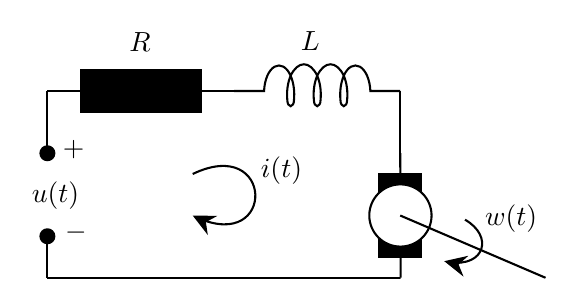
\begin{tikzpicture}[x=0.75pt,y=0.75pt,yscale=-1,xscale=1]
%uncomment if require: \path (0,300); %set diagram left start at 0, and has height of 300

%Shape: Resistor [id:dp2881948360242216] 
\draw  [fill={rgb, 255:red, 0; green, 0; blue, 0 }  ,fill opacity=1 ] (56.2,40) -- (113.8,40) -- (113.8,60) -- (56.2,60) -- (56.2,40) -- cycle (40,50) -- (56.2,50) (113.8,50) -- (130,50) ;
%Straight Lines [id:da984787262080848] 
\draw    (40,110) ;
%Straight Lines [id:da14919346198631556] 
\draw    (40,50) -- (40,80) ;
\draw [shift={(40,80)}, rotate = 90] [color={rgb, 255:red, 0; green, 0; blue, 0 }  ][fill={rgb, 255:red, 0; green, 0; blue, 0 }  ][line width=0.75]      (0, 0) circle [x radius= 3.35, y radius= 3.35]   ;
%Shape: Inductor (Air Core) [id:dp807027771192479] 
\draw   (130,50) -- (144.4,50) .. controls (144.61,44.57) and (146.61,39.93) .. (149.43,38.31) .. controls (152.26,36.69) and (155.35,38.41) .. (157.2,42.66) .. controls (158.63,45.97) and (159.21,50.25) .. (158.8,54.41) .. controls (158.8,56.03) and (158.08,57.34) .. (157.2,57.34) .. controls (156.32,57.34) and (155.6,56.03) .. (155.6,54.41) .. controls (155.19,50.25) and (155.77,45.97) .. (157.2,42.66) .. controls (158.86,39.13) and (161.18,37.13) .. (163.6,37.13) .. controls (166.02,37.13) and (168.34,39.13) .. (170,42.66) .. controls (171.43,45.97) and (172.01,50.25) .. (171.6,54.41) .. controls (171.6,56.03) and (170.88,57.34) .. (170,57.34) .. controls (169.12,57.34) and (168.4,56.03) .. (168.4,54.41) .. controls (167.99,50.25) and (168.57,45.97) .. (170,42.66) .. controls (171.66,39.13) and (173.98,37.13) .. (176.4,37.13) .. controls (178.82,37.13) and (181.14,39.13) .. (182.8,42.66) .. controls (184.23,45.97) and (184.81,50.25) .. (184.4,54.41) .. controls (184.4,56.03) and (183.68,57.34) .. (182.8,57.34) .. controls (181.92,57.34) and (181.2,56.03) .. (181.2,54.41) .. controls (180.79,50.25) and (181.37,45.97) .. (182.8,42.66) .. controls (184.65,38.41) and (187.74,36.69) .. (190.57,38.31) .. controls (193.39,39.93) and (195.39,44.57) .. (195.6,50) -- (210,50) ;
%Straight Lines [id:da4172890730978652] 
\draw    (210,50) -- (210,80) ;
%Straight Lines [id:da41804052897654165] 
\draw    (210.19,139.97) -- (210,140) ;
%Straight Lines [id:da21945983640661326] 
\draw    (40,140) -- (210,140) ;
%Straight Lines [id:da6747977271877703] 
\draw    (40,120) -- (40,140) ;
\draw [shift={(40,120)}, rotate = 90] [color={rgb, 255:red, 0; green, 0; blue, 0 }  ][fill={rgb, 255:red, 0; green, 0; blue, 0 }  ][line width=0.75]      (0, 0) circle [x radius= 3.35, y radius= 3.35]   ;
%Curve Lines [id:da974518805778978] 
\draw    (110,90) .. controls (149.2,71.13) and (150.46,127.9) .. (112.38,111.12) ;
\draw [shift={(110,110)}, rotate = 386.57] [fill={rgb, 255:red, 0; green, 0; blue, 0 }  ][line width=0.08]  [draw opacity=0] (10.72,-5.15) -- (0,0) -- (10.72,5.15) -- (7.12,0) -- cycle    ;
%Curve Lines [id:da9288185134435896] 
\draw    (241.2,112) .. controls (255.07,119.98) and (250.71,134.82) .. (233.95,132.51) ;
\draw [shift={(231.2,132)}, rotate = 373.03999999999996] [fill={rgb, 255:red, 0; green, 0; blue, 0 }  ][line width=0.08]  [draw opacity=0] (10.72,-5.15) -- (0,0) -- (10.72,5.15) -- (7.12,0) -- cycle    ;
%Shape: Rectangle [id:dp3201848725409655] 
\draw  [fill={rgb, 255:red, 0; green, 0; blue, 0 }  ,fill opacity=1 ] (200,90) -- (220,90) -- (220,130) -- (200,130) -- cycle ;
%Shape: Output [id:dp8772052388475995] 
\draw  [fill={rgb, 255:red, 255; green, 255; blue, 255 }  ,fill opacity=1 ] (210.05,94.99) .. controls (218.33,94.97) and (225.07,101.66) .. (225.09,109.94) .. controls (225.12,118.22) and (218.43,124.95) .. (210.14,124.98) .. controls (201.86,125) and (195.12,118.31) .. (195.09,110.03) .. controls (195.07,101.75) and (201.76,95.02) .. (210.05,94.99) -- cycle (210,80) -- (210.05,94.99) (210.19,139.97) -- (210.14,124.98) ;
%Straight Lines [id:da7015471005162024] 
\draw    (210,110) -- (280,140) ;

% Text Node
\draw (78,20.4) node [anchor=north west][inner sep=0.75pt]    {$R$};
% Text Node
\draw (160.6,20) node [anchor=north west][inner sep=0.75pt]    {$L$};
% Text Node
\draw (46,72.4) node [anchor=north west][inner sep=0.75pt]    {$+$};
% Text Node
\draw (47,112.4) node [anchor=north west][inner sep=0.75pt]    {$-$};
% Text Node
\draw (31,92.4) node [anchor=north west][inner sep=0.75pt]    {$u( t)$};
% Text Node
\draw (141.4,80.4) node [anchor=north west][inner sep=0.75pt]    {$i( t)$};
% Text Node
\draw (249.4,103.2) node [anchor=north west][inner sep=0.75pt]    {$w( t)$};


\end{tikzpicture}
